\chapter{Preliminares} % (fold)
En  este  capítulo  se hablará  sobre  el  correo  electrónico  y  algunos  de  los intermediarios que hacen posible que este servicio sea usado en toda la red de  internet, también  se describirán las  amenazas a  las  que  se   enfrenta  este  servicio para  hacer  llegar  información  de  un  usuario  a  otro  de  una  manera  segura  y  cuales  han 
sido   las   respuestas   de   los   proveedores   de   servicio   de   correo   electrónico   para proporcionar dicha seguridad a los usuarios. 


\section{Correo electrónico} 
El  correo  electrónico  es  el  servicio  de  internet  por  el cual  se  pueden  enviar  mensajes entre dos usuarios que cuenten con este servicio. El correo electrónico o “e-mail”
 por sus siglas en inglés, basa su funcionamiento en las oficinas postales. Tomando esa analogía se puede afirmar  que  los  usuarios  tienen  cartas  (mensajes  de  correo  electrónico)  que desean  enviar  a  otros  usuarios;  estas  son  enviadas  a 
las  oficinas  postales (servidores de correo electrónico) donde se almacenan con otras cartas que van dirigidas a otros usuarios en diferentes ciudades; estas oficinas las envían a otras 
oficinas   si es  necesario;  y por  último estas se  encargan de colocar el mensaje en el  buzón del usuario correspondiente (buzón  de  correos  electrónicos).\\
Para poder entender la comunicación en correo electrónico se necesitan definir los siguientes conceptos:
\begin{itemize}
\item \textbf{Mensaje de correo electrónico}
Los  mensajes  de  correo  electrónico  al  igual  que  las  cartas  tienen  la  dirección  del receptor, la dirección del emisor y el cuerpo del mensaje, pero a diferencia de las cartas 
los correos electrónicos son enviados por internet y necesitan sus propios formatos. Para  poder  enviar  un  mensaje  de  correo  electrónico  es  necesario  tener  los siguientes  elementos 
como mínimo.\\ 
\textit{Dirección  del  remitente}:  Esta  dirección  se  compone  por  dos  elementos  importantes,  el primero es el nombre de usuario seguido de un carácter “@”, el segundo elemento es 
el dominio donde está alojado el servicio de correo electrónico.\\ 
\textit{Direcciones  de  los  receptores}:  En  un  correo  electrónico  debe  haber  al  menos  una dirección  de  receptor  para  ser  enviado,  esta    tiene  la  misma estructura que la dirección del remitente.     \\  
\textit{Contenido  del  mensaje}:  Es  el  texto  que  se  desea  transmitir entre  el  remitente  y  el receptor. \\ 
El mensaje de correo electrónico cuenta con más elementos pero estos son opcionales y se pueden consultar en el RFC 2821 extensión MIME.\cite{rfc2821}
\item \textbf{Dominio de internet}\\
Es un nombre que identifica a los diferentes dispositivos interconectados en una red sin la  necesidad  de  aprenderse  un  número  de  red.  Estos  dispositivos  pueden  proporcionar 
diferentes servicios como el servicio de correo electrónico. 
\item \textbf{Buzón de correo electrónico}
Un  buzón  de  correo  electrónico  es  un  espacio  virtual  proporcionado  por  el  servicio  de correo electrónico que sirve para almacenar los mensajes enviados y recibidos. 
\item \textbf{Usuario de correo electrónico}
Se  le  conoce  como  usuario  de  correo  electrónico  a  la  persona  que  se  registra  en  un dominio  para  obtener  los  servicios  de  mensajería  proporcionados  por  un  servidor  de correo electrónico. 
\item \textbf{Cliente de correo electrónico}
El  cliente  de  correo  electrónico  es  una  interfaz  por  la  cual  el  usuario  de  correo  electrónico puede administrar sus mensajes enviados y recibidos. \\
El cliente de correo electrónico puede ser de diferentes tipos como son: 

 \textit{Cliente de correo electrónico para la pc}:
Estos clientes de correo electrónico son instalados en una computadora y es configurado para sincronizarse con un servidor de correo electrónico cada cierto tiempo o cuando el usuario se lo indique. 
Una  de  las  principales  características  de  éste  cliente  de  correos  es  la  capacidad  de descargar los mensajes del servidor a la computadora para ser leídos sin la necesidad de tener  una  conexión  de  internet  y  en  cuanto  tiene  conexión  con  el  servidor  otra  vez 
descarga los nuevos mensajes y envía los que se tienen pendientes en la computadora. 

 \textit{Cliente de correo electrónico web}:
Los  clientes  web  necesitan  un  explorador  de  internet  y  una  conexión  permanente  a  la red  para  que  funcione,  estos  clientes  normalmente  son  proporcionados  por  el  mismo servidor de correo electrónico y nunca descarga los correos en la computadora donde son utilizados. 

 \textit{Cliente de correo electrónico para móviles}:
Un  cliente  de  correo electrónico  móvil  se  caracteriza  por  ser una  aplicacion  instalada  en  un dispositivo  móvil. Esta aplicación descarga una copia temporal de los últimos mensajes recibidos.  

\item \textbf{Servidor de Correo electrónico}
Un servidor de correo electrónico es un programa que se encarga de enviar y recibir los mensajes de correo electrónicos de sus usuarios registrados, este servidor puede recibir 
mensajes  de  usuarios  de  otros  servidores  de  correos  que  sean  dirigidos  a  sus  usuarios registrados. \\
Este  servidor  tiene  que  seguir  algunos  estándares  que  existen  en  internet  para  el  envío(protocolo smtp)  y recepción(protocolo pop3 o imap) de mensajes de correo electrónico. 
\item \textbf{Protocolo SMTP}
El protocolo SMTP significa “protocolo para transferencia simple de correo” o “Simple Mail  Transfer  Protocol”   por  sus  siglas  en  inglés,  el  cual  se  encarga  de  enviar  los 
mensajes de correo electrónicos entre dispositivos que se encuentran interconectados en la  red  o  en  internet.  Este  protocolo  solo  se  utiliza  para mandar  los  mensajes  entre 
servidores  o  entre  el  usuario  emisor  y  su  servidor  de  correo  electrónico.  Podemos revisar el protocolo completo en el RFC5321\cite{RFC5321}.
\item \textbf{Protocolo POP3}
Este protocolo se encarga de descargar los mensajes del servidor a un cliente de correo electrónico  que  el  usuario  haya  configurado  previamente.  Una  de  las  características  es 
que  solo se sincroniza para  la descarga de  los  mensajes de  correo y  no deja una copia de seguridad en el servidor de correo electrónico. Podemos consultar el funcionamiento detallado en el RFC1939 \cite{1939}.
\item \textbf{Protocolo IMAP}
Este  protocolo,  al  igual  que  el  protocolo  POP3,  se  encarga  de  la descarga  de  los mensajes  del  servidor  a  un  cliente  de  correo  electrónico  con  la  diferencia  de  que  la 
sincronización  entre  el  servidor  y  el  cliente   es continua,  manteniendo  una  copia  de  seguridad  en  el  servidor.  Con  este  protocolo  es 
posible tener varios clientes de correo configurados con la misma  cuenta y los cambios que se realicen en cualquiera de los clientes de correo se verán reflejados en el servidor 
y  en  los  diferentes  clientes  sincronizados.  Este  protocolo  puede  ser  consultado  en  el RFC 6851\cite{6851}.\\ 


\end{itemize}

Como se ha podido ver en el presente documento, el servicio de correo electrónico es un  canal  de  comunicación  que  se  ayuda  de  varios  elementos  para  completar  la 
comunicación  entre  dos  usuarios  de  correo  electrónico,  sin importar que  estén registrados en 2 servidores de correo diferentes. Pero 
para poder entender por completo el  comportamiento  de  este  servicio  se tiene  que  definir  ciertas  características  de  este servicio. 
\\
Este servicio establece una comunicación no orientada a conexión, lo que significa que el  receptor  no  necesita  estar  conectado  al  servicio  de  correo  electrónico  para  recibir  el mensaje en su buzón de correo electrónico. 
\\
Los mensajes enviados por medio del correo electrónico transitan por el   internet   como archivos  en  texto  plano,  esto  quiere  decir  que  cualquiera  que  tenga  una  copia  del 
mensaje puede abrir el correo            electrónico    y    leer    el    mensaje    siguiendo    la estructura del protocolo SMTP. 
\\
Además  de  mandar  mensajes  tiene  la  facultad  de  enviar  archivos  multimedia  en  el mismo mensaje de correo electrónico, esta característica ha sido explotada bastante por empresas   privadas   y   de   gobierno   para   tener   comunicados   a   sus empleados, departamentos, proveedores, socios, etc. 
\\
El  correo  permite  enviar  el  mismo  mensaje  a  más  de  un  usuario  sin  la  necesidad  de hacer un mensaje para cada usuario, esto lo han       utilizado     muchas     empresas     de 
publicidad para hacer publicidad a gran   escala y a muy bajo costo, a este servicio se le llama SPAM. 
\\
Este  medio  de  comunicación  es  bastante  rápido  ya  que  se  estima  que  un  mensaje  de correo  electrónico  tiene  que  llegar  a  su  destino  a  más  tardar  en  5  minutos,  no 
importando la ubicación geográfica del        servidor de correo electrónico. 
\\
Las características mencionadas  dan a notar que el correo electrónico tiene una baja seguridad al momento de enviar los mensajes, ya que la información que se manda es 
sumamente fácil de leer por cualquiera que pueda tener una copia del mensaje. Si se toma en cuenta que un mensaje tiene que saltar 
por  varios  servidores  antes  de  llegar  a  su  destino,  es  fácil  suponer  que  se puede interceptar una copia del mensaje en el envío de servidor a servidor. 
\\
Por  estos  motivos  los  servidores  de  correo  electrónico  han implementado  diversos candados  de  seguridad  para  blindar  la  transferencia  de  mensajes  entre  servidores.  Una 
de  las  maneras  que  han  encontrado  para  proporcionar  dicha seguridad  ha  sido  a través de la implementación de técnicas criptográficas. 
\\


\section{Criptografía}


El objetivo fundamental de la criptografía es establecer una comunicación segura entre dos usuarios, usualmente esta comunicación es representada con Alicia y Bob, que son los interlocutores en un canal de comunicación y a una tercera persona que es el adversario, Oscar, que ataca la comunicación para obtener información. \\
Cuando Alicia manda un mensaje a Bob se le llama “texto en claro” y si Oscar intercepta el mensaje puede leer su contenido sin problemas. Ahora si Alicia cifra el texto en claro usando una clave, ella obtiene un texto cifrado el cual es enviado por el canal de comunicación a Bob, si Oscar intercepta este mensaje ya no podra leerlo porque no sabe como pasar del texto cifrado al texto el claro, pero Bob si puede recuperar el texto en claro, por que él sí conoce la clave de cifrado.\cite{stinson} Ver figura \ref{fig:1-2-1}\\

Formalmente la criptografía es el estudio de técnicas matemáticas relacionadas con la seguridad para proveer, confidencialidad, integridad y autenticación. Estas técnicas están destinadas a alterar las representaciones lingüísticas de ciertos mensajes con el fin de hacerlos ininteligibles a receptores no autorizados.\cite{cri}\\\\
Estos servicios se describen a continuación:
\begin{itemize}
 \item \textbf{Confidencialidad}:  La  información  sólo es  accesible  sólo  para  aquéllos  que  están autorizados.
 \item \textbf{Integridad}:  La información sólo puede ser creada y modificada por quien esté autorizado a hacerlo.
 \item \textbf{Autenticación}: Se garantiza que el mensaje provino del aparente autor o fuente.
 \item \textbf{No repudio}:  Este servicio evita que las entidades en una conexión nieguen compromisos establecidos previamente.
\end{itemize}

Un sistema criptográfico es una quintupla $(\cal M,C,K,E,D)$ donde:

\begin{enumerate}
 \item $\cal M$ es el espacio finito de posibles mensajes en claro.
 \item $\cal C$ es el espacio finito de posibles mensajes cifrados.
 \item $\cal K$ es el espacio finito deposibles claves a utilizar.
 \item Para cada $K \in \cal K$, se tiene una regla $e_k\in \varepsilon$ y su correspondiente regla $d_k\in \cal D$. Donde $e_k :\cal P\rightarrow C$ y $d_k:\cal C\rightarrow P$ siendo funciones tales que $d_k(e_k(x))=x$ siendo $x$ un elemento del espacio de textos en claro $x\in\cal P$
\end{enumerate}



\subsection{Tipos de Ataques}
A  pesar  de  la  implementación  de  estas  técnicas  criptográficas  los  ataques  a  las comunicaciones  siguen  existiendo  y  estos  ataques  se  han  clasificado  dependiendo  de 
cuanta  información  tenga  disponible  el  adversario  para  poder  romper  el  cifrado.\cite{at} Los tipos de ataques son:
\begin{itemize}
 \item \textbf{Ataque con sólo texto cifrado(Ciphertext-only  attack)}: En este tipo de ataque el adversario tiene acceso sólo al texto cifrado, y no tiene acceso al texto plano, pero es el ataque más débil debido a la falta de información.
 \item \textbf{Ataque de texto plano(Known plaintext attack)}: En este tipo de ataque el adversario se supone que tienen acceso a la lista en un número limitado de pares de texto plano y el texto cifrado correspondiente.
 \item \textbf{Ataque de texto cifrado elegido(Chosen ciphertext attack)}: Este ataque se puede elegir los textos cifrados arbitrariamente y tener acceso a texto planos después de ser procesados. Para que este ataque se lleve a cabo es necesario tener el extremo receptor de la comunicación y acceso al canal de la comunicación.
 \item \textbf{Ataque de texto plano elegido(Chosen plaintext attack)}: Este ataque es capaz de elegir una serie de textos planos para ser cifrados y tener acceso al texto cifrado resultante. Esto le permite explorar cualquier área del espacio de  texto plano que desea y puede permitirle explotar el comportamiento no aleatorio que sólo aparecen con ciertos textos planos.
\end{itemize}




\subsection{Cifrado Simétrico}
Un sistema de cifrado simétrico es un tipo de cifrado que usa una misma clave para cifrar y para descifrar. Las dos partes que se comunican mediante el cifrado simétrico deben estar de acuerdo en la clave a usar de antemano. Una vez de acuerdo, el remitente cifra un mensaje usando la clave, lo envía al destinatario, y éste lo descifra usando la misma clave.\cite{sime}\\

\begin{figure}[H]
\centering
	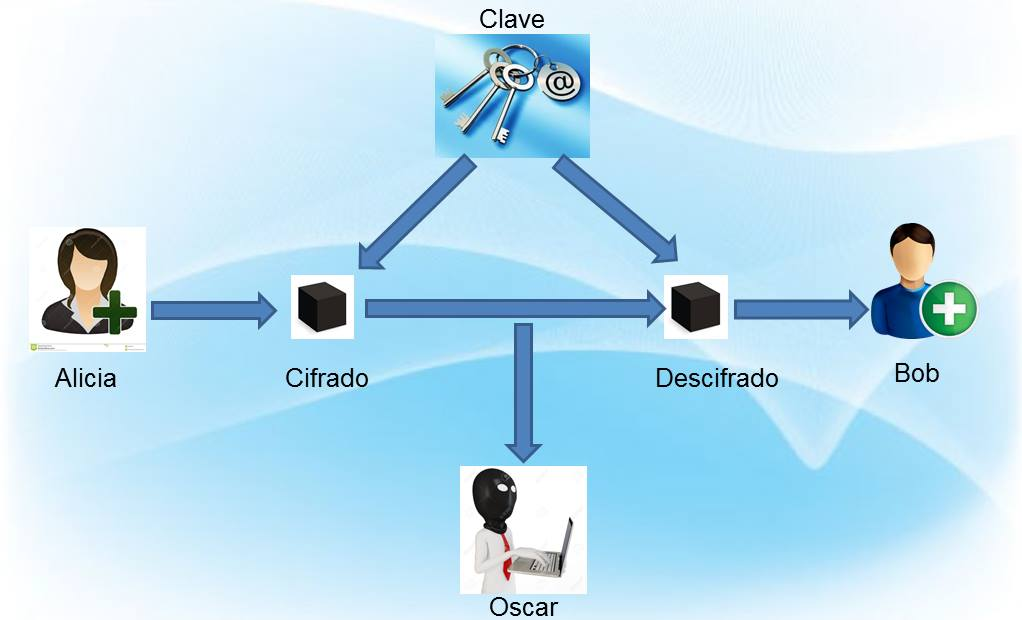
\includegraphics[width=10cm, height=5cm]{./images/simetrico.jpg}
	\caption{Diagrama cifrado simétrico}
	\label{fig:1-2-1}
\end{figure}

\subsection{Cifrado por bloques}
Este tipo de cifrado toma bloques de información del texto plano y produce bloques de información cifrados de un tamaño fijo, normalmente es del mismo tamaño que el bloque de información del texto plano. Los bloques de cifrado tienen que cumplir la condición de ser lo suficientemente grandes como para evitar ataques de texto cifrado, otra condición que se debe cumplir es que la asignación de bloques de entrada a bloques de salida es uno a uno para hacer el proceso reversible.\\
Formalmente un cifrado en bloque se considera que es seguro si se comporta como una permutación pseudoaleatoria fuerte, es decir, un cifrado de bloques es seguro si un adversario no puede distinguir su salida de una permutación elegida al azar.\\
Para hacer la asignación de bloques los algoritmos de cifrado utilizan sustituciones y permutaciones en los bloques de texto plano hasta obtener un texto cifrado.\\
La sustitución es el reemplazo de un bloque de $n$ bits por otro bloque de $n$ bits en un espacio de \(2^{k}\).\cite{bloc}\\
Los cifradores por bloques mas usados son:
\begin{itemize}
 \item Estandar de Cifrado de Datos DES (Data Encryption Standard)
 \item Estandar de cifrado Avanzado AES (Advanced Encryption Standard)
\end{itemize}


\subsection{Modos de operación}
Los modos de operacion fueron desarrollados para el algoritmo DES, estos fueron estandarizados en Diciembre de 1980. 
Cuando la informacion es cifrada usando la misma clave, surge una serie de problemas de seguridad. En esencia los modos de operacion son una técnica para mejorar el efecto criptografico de los cifradores por bloques.\cite{modes}\\\\
\textit{ECB}(Electronic codebook): Este modo de operación es probablemente el más simple de todos, el texto plano M está segmentado como $ M=M_1||M_2||...||M_m$ donde cada $M_i$ es un bloque de n bits. A continuación la funcion de cifrado $E_k$ se aplica por separado a cada bloque $M_i$. \\
A continuación tenemos el diagrama de este modo de cifrado.\\
\begin{figure}[h]
    \centering
    \begin{subfigure}[t]{0.5\textwidth}
        \centering
        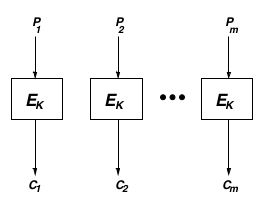
\includegraphics[height=1.7in]{./images/ecb1.png}
        \caption{Diagrama ECB Cifrado}
        \label{fig:1-3-1}
    \end{subfigure}%
    ~ 
    \begin{subfigure}[t]{0.5\textwidth}
        \centering
        \includegraphics[height=1.7in]{./images/ECB2.png}
        \caption{Diagrama ECB Descifrado}
        \label{fig:1-3-1}
    \end{subfigure}
    \label{fig:protocol}
\end{figure}


\textit{CBC}(Cipher-block chaining): Para este modo de operación la salida de un bloque de cifrado se introduce en el siguiente bloque de cifrado junto con el siguiente bloque del mensaje.\\

\begin{figure}[h]
    \centering
    \begin{subfigure}[t]{0.5\textwidth}
        \centering
        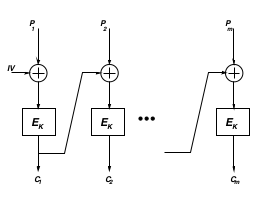
\includegraphics[height=1.7in]{./images/cbc1.png}
        \caption{Diagrama CBC Cifrado}
        \label{fig:1-4-1}
    \end{subfigure}%
    ~ 
    \begin{subfigure}[t]{0.5\textwidth}
        \centering
        \includegraphics[height=1.7in]{./images/CBC2.png}
        \caption{Diagrama CBC Descifrado}
        \label{fig:1-4-1}
    \end{subfigure}
    \label{fig:protocol}
\end{figure}

 \begin{figure}[H]
 \centering
	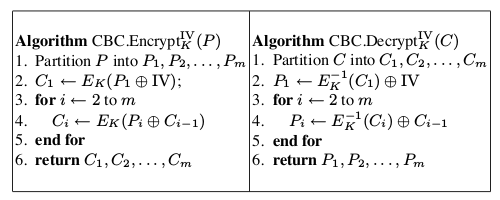
\includegraphics[width=14cm, height=6cm]{./images/pcbc.png}
	
\end{figure}

CBC toma como bloques de mensajes de entrada M y un vector de inicialización (IV). Durante el cifrado, la salida del i-ésimo bloque depende de los i-1 bloques anteriores. Así, el cifrado CBC es intrínsecamente secuencial.\\

\textit{CFB}(Cipher Feedback): En este modo de operación, los bloques de cifrado también están encadenados pero a la salida se produce de una manera muy diferente de la de CBC. Cada bloque de salida se le aplica XOR con el siguiente bloque de entrada.\\

\begin{figure}[h]
    \centering
    \begin{subfigure}[t]{0.5\textwidth}
        \centering
        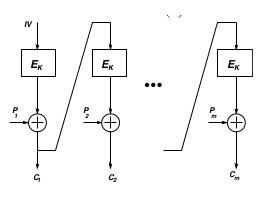
\includegraphics[height=1.7in]{./images/cfb1.png}
		\caption{Diagrama CFB Cifrado}
		\label{fig:1-5-1}
    \end{subfigure}%
    ~ 
    \begin{subfigure}[t]{0.5\textwidth}
        \centering
        \includegraphics[height=1.7in]{./images/CFB2.png}
		\caption{Diagrama CFB Descifrado}
		\label{fig:1-5-1}
    \end{subfigure}
    \label{fig:protocol}
\end{figure}

\begin{figure}[H]
\centering
	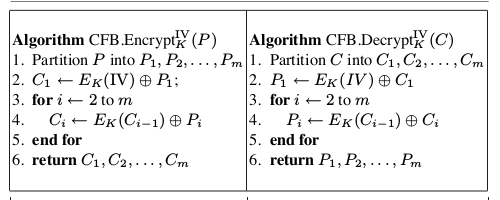
\includegraphics[width=14cm, height=6cm]{./images/pcfb.png}
	
\end{figure}


\textit{OFB}(Output feedback): En este modo de operación el IV se cifra varias veces para obtener un flujo de bytes aleatorios, el resultado de esto se aplica XOR con el bloque de texto plano mientras que el flujo de bytes aleatorios se usa como parámetro del siguiente bloque. A diferencia de los otros modos en OFB ninguna parte del texto claro entra directamente a cifrarse.

\begin{figure}[h]
    \centering
    \begin{subfigure}[t]{0.5\textwidth}
        \centering
        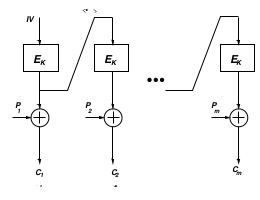
\includegraphics[height=1.7in]{./images/ofb1.png}
		\caption{Diagrama OFB Cifrado}
		\label{fig:1-6-1}
    \end{subfigure}%
    ~ 
    \begin{subfigure}[t]{0.5\textwidth}
        \centering
        \includegraphics[height=1.7in]{./images/OFB.png}
		\caption{Diagrama OFB Descifrado}
		\label{fig:1-6-1}
    \end{subfigure}
    \label{fig:protocol}
\end{figure}

\begin{figure}[H]
\centering
	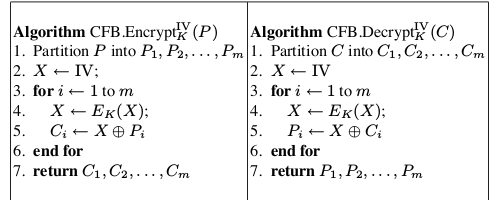
\includegraphics[width=14cm, height=6cm]{./images/pofb.png}
	
\end{figure}
\pagebreak
\section{Funciones Hash}
Las funciones hash son usadas pra construir una pequeña huella digital de la informacion, si la informacion es alterada tambien la huella digital es alterada. Esta caracteristica hace que las funciones hash sean ampliamente usadas para verificar la integridad de datos.\\
De manera formal, un funcion Hash es una Cuadrupla$(X,Y,K,H)$ donde:
\begin{enumerate}
 \item $X$ es un conjunto de posibles mensajes.
 \item $Y$ es un conjunto finito de posibles resúmenes de mensajes o etiquetas de autenticación.
 \item $K$, el espacio de claves, es un conjunto finito de posibles claves.
 \item Para cada $k\quad \epsilon\quad K$, existe una función hash $h_k\quad \epsilon\quad H$. Parac ada $h_k: X \longrightarrow Y$.
 \cite{stinson}
\end{enumerate}



\section{Aritmética Modular}
\textbf{Aritmética}:\\
En matemática, la aritmética modular es un sistema aritmético para clases de equivalencia de números enteros llamadas clases de congruencia.
La aritmética modular puede ser construida matemáticamente mediante la relación de congruencia entre enteros, que es compatible con las operaciones en el anillo de enteros: suma y multiplicación.
La aritmética modular se basa en una relación de equivalencia, y las clases de equivalencia de un entero a se denota con [a]n (o simplemente [a] si sobreentendemos el módulo.) $a\quad mod\quad n$. El conjunto de todas las clases de equivalencia se denota con $Zn = { [0]n, [1]n, [2]n,..., [n-1]n }.$
Un hecho importante sobre aritmética modular, cuando los módulos son números primos es el pequeño teorema de Fermat: si p es un número primo, entonces.\cite{modular}\\\\
Si $a$ es cualquier entero:\\\\
$a^p\equiv a(mod\quad p)$\\\\
Si $a$ es un entero no divisible entre $p$:\\\\
$a^{p-1}\equiv 1(mod\quad p)$\\\\
\textbf{Numeros primos}:\\
Los números primos son aquellos números enteros que sólo son divisibles por si mismos y por la unidad. Los numeros que no son primos se llaman compuestos, excepto el numero 1 que no se considera ni primo ni compuesto. En el libro IX Euclides demostró que existe una infinidad de numeros primos.\\\\
\textbf{Anillo}: Un anillo es un sistema algebraico formado por un conjunto no vacío y dos operaciones internas, llamadas usualmente suma y producto. El producto en un anillo no necesariamente tiene una operación inversa definida, aun que puede ser definida por su inverso multiplicativo.\cite{anil}\\\\ 
\\
\textbf{Zp}:\\
Sea $Zp$ un conjunto de elementos con dos operaciones binarias, suma y multiplicación y $p$ sea un numero primo. Dicho conjunto tendra estructura de anillo si satisface.\cite{zp}
\begin{itemize}
 \item $Zp$ es asociativa bajo la multiplicación.\\\\
 $(a . b) . c  =  a . (b . c)$
 \item La multiplicación es distributiva respecto a la suma.\\
 Para $a,b,c\quad\epsilon\quad Zp$\\\\
 $a.(b+c)=a.b+a.c$\\\\
 $(a+b).c=a.c+b.c$
\end{itemize}


\textbf{Euclides Extendido}:\\
Una de las técnicas básicas de la téoria de números es el algoritmo de Euclides, que es un procedimiento simple para la determinación del maximo comun 	divisor de dos números enteros positivos.\\
$b$ se define como un divisor de $a$ si $a=mb$ para algun $m$ tal que $a$,$b$ y $m$ son numeros enteros.
Utilizaremos la notación $gcd (a, b)$ que significa el máximo común divisor de a y b.\\
Supongamos que tenemos los numeros enteros $a$, $b$ de tal manera que $d=gcd(a,b)$, suponiendo que $a\geq b > 0$. Ahora dividir $a$ entre $b$ y aplicando el algoritmo de la división:\\\\
$a=q_1b++r_1$   donde $0\leq r_1<0$.\\\\
Sucede que si $r_1=0$ entonces $gcd(a,b)=b$ pero si $r_1\neq 0$. Se procede a resolver $gcd(b,r_1)$ y se aplica el algoritmo de divicion.\\\\
$b=q_2r_1+r_2$\\\\
Del mismo modo si $r_2=0$ entonces $gcd(b,r_1)=r_1$ y si $r_2\neq 0$, entonces continua el proceso de divicion con $gcd(r_1,r_2)$. El resultado es el siguiente sistema de ecuaciones:\\\\
$a=q_1b+r_1$\\
$b=q_2r_1+r_2$\\
$r_1=q_3r_2+r_3$\\
$.$\\
$.$\\
$.$\\
$r_{n-2}=q_nr_{n-1}+r_n$\\
$r_{n-1}=q_{n+1}r_n+0$\\
$gcd(a,b)=r_n$\\\\
Para los enteros $a$, $b$ el algoritmo de Euclides Extendido no solo calcula el maximo comun divisor $d$ si no que adicionalmente se calculan los numeros $x$, $y$ tal que.\\\\
$ax+by=d=gcd(a,b)$\\
Con base en esto el calculo del algoritmo de euclides extendido para $(x,y,d)$. Dado  $a$ y $b$ usamos la secuencia de diviciones indicada en las ecuaciones anteriores, y suponemos que en cada paso podemos encontrar $i$ enteros $x_i$ y $y_i$ que satisfagan la ecuacion $r_i=ax_i+by_i$.\\
Tenemos la secuencia:\\
$a=q_1b+r_1$\\
$b=q_2r_1+r_2$\\
$r_1=q_3r_2+r_3$\\
$.$\\
$.$\\
$.$\\
$r_{n-2}=q_nr_{n-1}+r_n$\\
$r_{n-1}=q_{n+1}r_n+0$\\\\
De esta secuencia podemos reordenar los terminos de la forma:\\
$r_n=r_{n-2}-r_{i-1}q_i$ ... (1.1)\\
Además, en filas $i-1$ e $i-2$ nos encontramos con los valores:\\
$r_{i-2}=ax_{i-2}+by_{i-2}$ y $r_{i-1}=ax_{i-1}+by_{i-1}$\\
Y sustituimos estas en la ecuacion (1.1) quedando.\\
$r_i=a(x_{i-2}-q_ix_{i-1})+b(y_{i-2}-q_iy_{i-1})$
\cite{modes}\\

\section{Polinomio de Lagrange}
 El polinomio de Lagrange, llamado así en honor a Joseph-Louis de Lagrange, es una forma de presentar el polinomio que interpola un conjunto de puntos dado. Este genera una aproximacion a una funcion dependiendo de los puntos que se introduscan.\cite{stinson}\\\\
 
 Dado un conjunto de $k + 1$ puntos\\\\
 $(x_0,y_0),...,(x_k,y_k)$\\\\
 donde todos los $x_j$ se asumen distintos, el polinomio interpolador en la forma de Lagrange es la combinación lineal.
 \begin{equation}
  L(x)=\sum_{j=0}^{k}y_jl_j(x)
 \end{equation}
 \\\\
 de bases polinómicas de Lagrange\\\\
 \begin{equation}
  l_j=\prod_{i=0,i\neq j}^{k}\frac{x-x_i}{x_j-x_i}=\frac{x-x_0}{x_j-x_0}...\frac{x-x_{j-1}}{x_j-x_{j-1}}\frac{x-x_{j+1}}{x_j-x_{j+1}}...\frac{x-x_k}{x_j-x_k}
 \end{equation}
El uso del Polinomio de Lagrange nos permite calcular de manera mas rapida un sistema de ecuaciones de la forma $a_0+a_1.x^1+...+a_n.x^n$.
